\section{Exploring the need for realism in client-side emulation}\label{summary:realism}

In this section, we aim to delve deeper into the implications of our methodology for the optimization of \gls{WCA}.
In particular, we wish to explore the impact improving the realism of the client-side emulation has on the potential for optimization of the applications under evaluation.
We approach this question by developing an improved, more detailed version of our model of human behavior in \gls{WCA} used in the EdgeDroid tool, which we then incorporate into our methodology along with a mathematical framework to study the potential for optimizing \gls{WCA} applications. 

Our work in \cref{paper:olguinmunoz2018demoscaling,paper:olguinmunoz2019edgedroid} has used a model that emulates a rigid and unyielding human who makes no mistakes and is not affected by low responsiveness in the system.
However, this is not an accurate representation of real human behavior, and a more realistic human model must take into consideration the perceived feedback latency and its effects on human reactions.
In order to develop a more accurate human model in the context of \gls{WCA}, we first conduct an experimental study that measures human performance in different scenarios, taking into account the impact of system latency on the behavior of humans.
The results of this study serve as the foundation for building a more representative model of human behavior.

Once we have established a more accurate model of human behavior, we can explore its implications for the optimization of \gls{WCA} through our methodology.
By improving the realism of our model of human behavior, we aim to gain novel understanding of the challenges involved in optimizing \gls{WCA} and how our methodology can be effectively applied to address these.
This research highlights the importance of the realism of emulations as  crucial factor in the application of our methodology.

\subsection{Definitions relating to the operation of \glsfmtshort{WCA} applications}

In order to more easily and accurately discuss the implications of our methodology for \gls{WCA}, we first characterize these applications and provide some definitions relating to their operation.
We focus in particular on \emph{step-based} \gls{WCA}, i.e.\ assistance applications which have as their goal the guidance of a user through a task, using a series of instructions.

As discussed above, \glspl{WCA} track the state of the real world through sampling of inputs, most commonly of video feeds.
In step-based \glspl{WCA}, the state in question refers to the progress of some arbitrary, sequential task, such as the assembly of a LEGO model or of a piece of IKEA furniture~\cite{chen2018application}.
We will formally define \emph{task} as a well-defined sequence of instructions to be performed in order to achieve a final goal state, and further define a \emph{step} within a task as a specific action to be performed by the user, described by a single instruction.
A step begins when the corresponding instruction is provided to the user, and ends when the instruction for the next step is provided;
the time interval between these two events will be referred to as the \emph{step duration}.

\begin{figure}
    \centering
    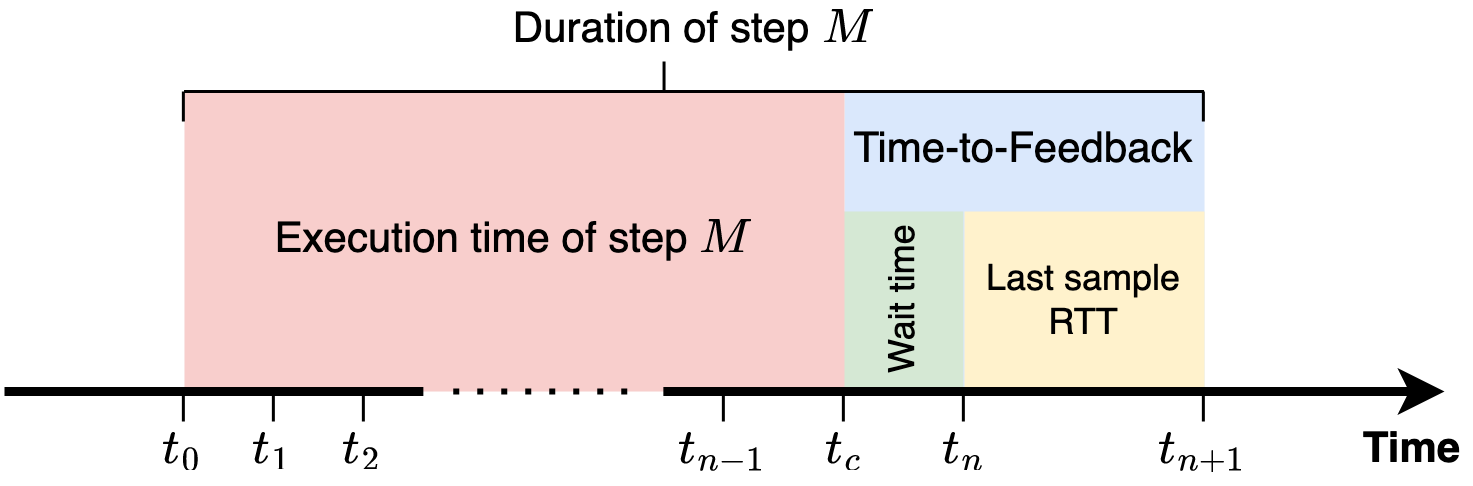
\includegraphics[width=.9\textwidth]{publications/2023EdgeDroid2/figs/step_time}
    \caption[]{%
        Breakdown of a step in a \gls{WCA} into its timing components.
        \ensuremath{t_k | k \in \{1, \ldots, n \}} correspond to sampling instants.
        \ensuremath{t_0} indicates the instant at which the instruction for step \ensuremath{M} is provided to the user and the first sample for said step is captured.
        The instruction for step \ensuremath{M + 1} is provided at \ensuremath{t_{n+1}}.
        Finally, \ensuremath{t_c} marks the instant at which the user finishes the instruction, and \ensuremath{t_n} the instant of capture of the first sample after the instruction has been completed;
        this sample therefore also corresponds to the final sample of step \ensuremath{M}.
        Figure originally included in \cref{paper:olguinmunoz2023realistic}.
    }\label{fig:wcastep}
\end{figure}

In the following, please refer to \cref{fig:wcastep}.
\ensuremath{\{ t_0, t_1, \ldots, t_{n + 1} \}} corresponds to a series of discrete and sequential sampling instants, such that \ensuremath{t_0} corresponds to the instant at which the instruction for step \ensuremath{M} is provided and the first sample of the step is taken.
\ensuremath{t_n} corresponds to the instant at which the final sample of step \ensuremath{M} is taken;
this sample is the first sample to capture the finished state of the step.
At this point, the application transitions to the next step \ensuremath{M + 1}, and thus \ensuremath{t_{n + 1}} is the instant at which the next instruction is provided and step \ensuremath{M + 1} begins.
We will also refer to the interval \ensuremath{t_{n + 1} - t_n} as the \emph{last sample \gls{RTT}}.

\glsreset{TTF}%
From this characterization, we can define key variables relating to human behavior with respect to the sampling behavior of these applications.
However, we first note that the combination of the characteristic of seamless interaction with the context of the user described in \cref{sec:background:wca} and in \cref{fig:wca:operation}, combined with the sampling behavior described above, lead to an interesting consequence for the perception of responsiveness in \gls{WCA}.
The only points in time at which a user can consciously notice and interact with the application is whenever they are \emph{expecting} feedback.
A corollary of this is that these are therefore also the \emph{only} points in time at which users can notice changes in system responsiveness.
If we understand \ensuremath{t_c} as the point in time at which the user finishes executing the instruction for step \ensuremath{M}, then
\begin{inlineenum}
    \item \ensuremath{t_c - t_0} corresponds to the \emph{step execution time}, that is, the time it has taken the user to complete the instruction
    \item \ensuremath{t_n - t_c} is the \emph{wait time}, an interval of time during which the task has been finished, but no sample capturing the new state has been taken yet
    \item finally, the interval \ensuremath{t_{n + 1} - t_c} we call \emph{\gls{TTF}}, and refers to the time the user spends waiting for a new instruction.
\end{inlineenum}
These values are key to understanding human perception of responsiveness in these systems, and therefore also to the optimization of resource consumption in \gls{WCA}.
We will refer to them extensively in \cref{chap:contributions}.

%\subsection{Mechanisms relating human behavior to system responsiveness}
%
%The question of how people respond to delay in a computer system is grounded in how people perceive time.
%Time perception has been described as regulated by an attentional gate that, when opened, starts a cognitive pulse counter~\cite{zakay1995attentional,zakay1996role}.
%More recent research indicates, however, that duration perception is highly malleable and the result of multiple timing mechanisms found in overlapping, flexible neural systems~\cite{bruno2016multiple,wiener2011multiple}.
%The estimation of an event's duration varies with context of various types
%\begin{inlineenum}[label={(\roman*)}, before=\unskip{: }, itemjoin={{; }}, itemjoin*={{; and }}]
%\item events subsequent to a long or short interval are contracted or extended, respectively~\cite{heron2012duration}
%\item repeated events tend to be perceived as shorter than novel ones~\cite{matthews2011stimulus}
%\item arousal can expand durations~\cite{droit_volet2011emotion}.
%\end{inlineenum}
%
%Expectations play a critical role in time perception as well~\cite{zakay1995attentional,zakay1996role}.
%It has been shown that people have a general tendency to be hypersensitive to delays in worse-than-expected states, and under-sensitive to meeting or exceeding expectations~\cite{loewenstein1992anomalies}.
%Accordingly, failures to meet expected fast response times tend to be experienced as highly negative, whereas fast latencies are not noticed.
%Violations of expectancy have a strong impact on the acceptability of computer systems.
%Users of a computer system anticipate the latency for events, for which the standards only become more stringent as systems improve in response time.
%In immersive systems like \gls{WCA}, which aim to provide seamless interaction, delays are particularly noticeable.
%
%It has long been recognized that slow system response times can undermine cognitive processing, slow the pace of users, and lead to stereotyped behavior and errors, as well as cause negative emotional consequences~\cite{dabrowski201140}.
%However, standards for what constitute tolerable delays have changed dramatically compared to three decades ago, when delays on the order of \SI{10}{\second} were deemed acceptable~\cite{nielsen1994usability, shneiderman2016designing, seow2008designing}.
%Today's user context, and \gls{WCA} in particular, often demand response times orders of magnitude shorter.
%
%For \gls{WCA} the acceptable range for latencies was explored by Chen et al.~\cite{chen2017empirical}, by constructing assistants for tasks with a range of time constraints, including step-by-step tasks and more interactive contexts like playing Ping-Pong against a human opponent.
%They then proposed a latency tolerance zone according to the task demands.
%For an essentially self-paced task like LEGO assembly, they found two key ranges of latency; unnoticeable, \SIrange{0}{0.6}{\second}; and impaired, \SIrange{0.6}{2.7}{\second}.
%Beyond that, users could begin to show the negative outcomes previously catalogued~\cite{dabrowski201140}.
%
%While behavioral changes and negative interaction outcomes have been well documented in prior research on system delay, the specific mechanisms that mediate these outcomes are less well understood.
%These mechanisms could be cognitive or emotional in origin.
%
%A first possible explanation comes from research on cognitive and motor planning.
%Delay may move users from relatively automatic to more attention-demanding processing.
%Cognitive and motor tasks are commonly described as a hierarchical system, progressing from high-level goals to the sequence of commands that accomplishes them.
%As competency in a task increases, execution of the hierarchy becomes increasingly automated.
%Automatization has been described from a computational perspective in {Anderson's ACT-R}~model as the compiling of multiple productions into one~\cite{neves1981knowledge}.
%Neural measurements indicate that with automaticity, control moves from frontal brain areas to more posterior ones~\cite{jeon2015degree,puttemans2005changes}, and similar distinctions have been related to temporal processing~\cite{lewis2003distinct,koch2009neural,lee2019limiting}.
%
%Although activities guided by a \gls{WCA} are not simple motor actions, immediate feedback after each of a series of repeated actions should promote development and automatic execution of a hierarchical plan.
%Delays, in contrast, would disrupt such a plan through the loss of automated control~\cite{lee2019limiting}.
%
%A second, alternative explanation of delay effects appeals to emotional systems rather than cognitive processes.
%As users of a system become emotionally aroused by delay, they may be subject to generalized arousal, causing decrements in performance~\cite{lee2019limiting}.
%
%Finally, a third potential explanation of delay effects is what has been called ``ego depletion'', the notion that expending effort on self-control eliminates resources needed for further effort~\cite{baumeister74tice,lin2020strong}.
%
%The various processing accounts of delay effects predict different outcomes, which we will consider in the context of the current data.
%If delay increases attentional demands on cognitive processes, responses should be slowed and errors expected, particularly on time-critical tasks.
%Generalized arousal triggered by emotional stress from delay should emerge in physiological measures, such as increased heart rate or skin conductivity.
%Arousal can also reduce movement smoothness or add erratic gestures~\cite{pijpers2003anxiety}.
%Ego depletion has been found to produce premature responses culminating in error~\cite{lin2020strong}, or to lead to abandoning a task entirely~\cite{baumeister74tice}.
%
%Over-arching prescriptions for tolerable system response time have not tended to take into account individual differences in users with respect to salient variables like cognitive ability or personality.
%Relevant research can be found in studies of delay discounting, the tendency to devalue rewards for which one must wait.
%High discounting rates, indicative of waiting intolerance, have been associated with negative social and academic outcomes.
%Hirsh et al.~\cite{hirsh2008delay} found that higher discounting was associated with extraversion among those with low cognitive function, whereas lower discounting was associated with emotional stability (low neuroticism) for people with high cognitive function.
%Among computer system users who tend to have relatively high cognitive ability (which presumably describes the present experimental population), this points to neuroticism as a personality factor that might modulate tolerance for waiting. Extraversion could also  be  a moderating factor among the broader target audience of \gls{WCA}, which are intended for relatively inexperienced users of an application.
%These and other measures of individual variation were considered here.


\subsection{Characterizing human behavior}

\Cref{paper:olguinmunoz2021impact} aims to investigate the effects of system responsiveness on human behavior in step-based \gls{WCA}.
This corresponds to the first step in extending our EdgeDroid tool for the benchmarking of \gls{WCA}, first introduced in \cref{paper:olguinmunoz2018demoscaling,paper:olguinmunoz2019edgedroid}, with a more realistic model of human behavior.
The study involved \num{40} undergraduate students who interacted with a \gls{WCA} application while the system responsiveness was systematically altered in real-time, and their behavioral and physiological reactions were recorded.
The study attempted to answer a number of core research questions relating to human behavior in the context of these applications.
These included
\begin{inlineenum}
    \item whether users change their actions in relation to system latency
    \item whether they show signals of arousal in physiological responses
    \item whether their responses to delay effects are mediated by cognition and/or emotion
    \item whether these effects are mediated by personality indicators
\end{inlineenum}.

We found that reduced system responsiveness induces additional behavioral slow-down in \gls{WCA} users, and this effect scales with the strength of the reduction in system responsiveness.
Furthermore, we note that humans tend to speed up as the task progresses;
however, as system responsiveness decreases, this effect is strongly dampened.
The effects of reduced system responsiveness on users linger for at least four steps after the system responsiveness improves, leading to longer execution times for steps immediately after a period of reduced responsiveness.
Finally, the trait of \emph{neuroticism}~\cite{john1999big} seems to play a significant role in modulating users' response to reduced responsiveness in \gls{WCA}.

\subsubsection{Methodology}

\begin{figure}[tb]
    \centering
    \begin{subfigure}[t]{.45\textwidth}
        \centering
        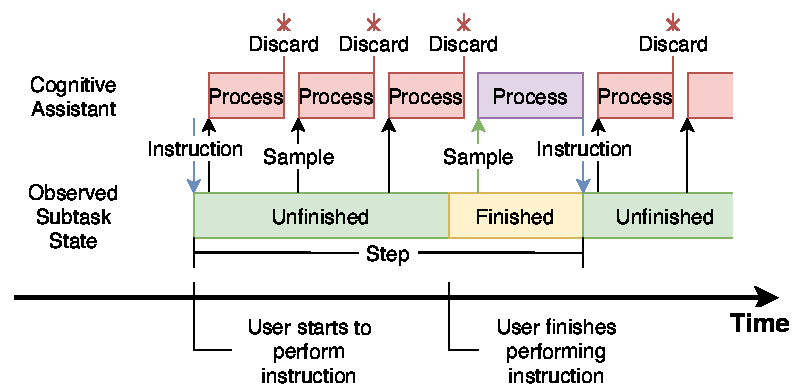
\includegraphics[width=\textwidth]{publications/2021ImpactDelayedResponse/Fig4a}
        \caption{}\label{sfig:regularwcaexec}
    \end{subfigure}%
    \hfill%
    \begin{subfigure}[t]{.45\textwidth}
        \centering
        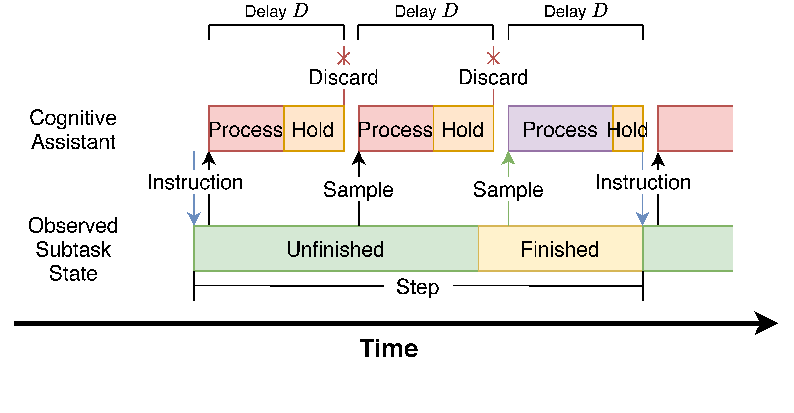
\includegraphics[width=\textwidth]{publications/2021ImpactDelayedResponse/Fig4b}
        \caption{}\label{sfig:delaywcaexec}
    \end{subfigure}
    \caption{%
        Comparison between normal task execution in the LEGO \gls{WCA}~\cite{chen2015early}~(\labelcref{sfig:regularwcaexec}) and modified task execution with delay in the experimental setup of \cref{paper:olguinmunoz2021impact}~(\labelcref{sfig:delaywcaexec}).
        In the experimental task, an additional variable segment of time is introduced immediately following the processing of the input frame in order to extend the perceived processing time of the input to a specific target interval of time denoted \emph{delay}.
        Figures originally published in \cref{paper:olguinmunoz2021impact}.
    }\label{fig:regularwca-vs-delaywca}
\end{figure}

We employed a version of the step-based \emph{Gabriel} cognitive assistant framework first introduced by \citeauthor{chen2018application}~\cite{chen2018application}.
The assistant was instrumented to capture key application and task performance metrics in real time, in particular step execution time.
Furthermore, the software was modified to allow for the real-time alteration of system responsiveness by extending the processing interval of each input to a temporarily fixed value denoted \emph{delay}.
This is illustrated in \cref{fig:regularwca-vs-delaywca}.
If, during a series of steps, delay was set to a value \ensuremath{\mathbb{D}}, the feedback for each input frame was provided to the user exactly a time interval \ensuremath{\mathbb{D}} after frame capture.
That is,
\begin{align}
    t_k - t_{k - 1} = \mathbb{D} \qquad \forall k \in [2, n + 1]
\end{align}
%Seven values were selected for \ensuremath{\mathbb{D}}: no added delay (which was referred to as \SI{0}{\second} delay), \SIlist{0.6;1.125;1.65;2.175;2.7;3.0}{\second}.
In order to fully characterize the resulting \emph{\glspl{TTF}} perceived by participants, we note that the instant of final frame capture for a step, \ensuremath{t_c} (and conversely the wait time \( \mathcal{W} \) of the step), can be assumed to be uniformly distributed in \( [t_{n - 1}, t_n] \), without loss of generality.
Thus the average \gls{TTF} for a step can be expressed as
\begin{align*}
    TTF = (t_{n + 1} - t_{n}) + \frac{1}{2}(t_n - t_{n - 1})
\end{align*}
which, for a step with a given delay \ensuremath{\mathbb{D}}, works out to\footnote{%
    The \num{0}/no-delay case was handled by calculating the empirical average frame \gls{RTT} for these steps, and using this value as the delay \ensuremath{\mathbb{D}}.
    This yielded an average \gls{TTF} of \SI{0.57}{\second} for these steps.
}
\begin{align}
    TTF &= \mathbb{D} + \frac{1}{2}\mathbb{D}\nonumber\\
    &= \frac{3}{2}\mathbb{D}
\end{align}
In the following, we will forgo the delay values and present results with respect to the adjusted \glspl{TTF}.

\begin{figure}[tb]
    \centering
    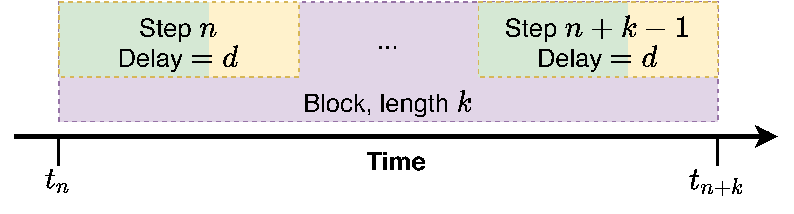
\includegraphics[width=.6\textwidth]{publications/2021ImpactDelayedResponse/Fig4c}
    \caption{%
        Structure of a \emph{block} in the experimental LEGO task.
        Figure originally published in \cref{paper:olguinmunoz2021impact}.
    }\label{fig:stepblock}
    \todo[inline]{This figure may need reworking for clarity.}
\end{figure}

\medskip
The \gls{WCA} task employed for this study corresponded to a modified and extended version of the LEGO assembly task introduced in~\cite{chen2015early}.
Unlike the original design of this task, in which the user is led through the assembly of a specific model, the modified LEGO task consisted of a pseudo-random sequence of steps instructing subjects to add or remove pieces.

We introduced an experimental design component denoted a \emph{block}, illustrated in \cref{fig:stepblock}, corresponding to a segment of consecutive steps subject to the same delay value.
To study the effects of a delay applied across multiple steps, we manipulated the length of blocks during the task. %, using values of \numlist[list-final-separator={, or }]{4;8;12} steps.
Furthermore, we defined a \emph{slice} as a continuous segment of \num{4} steps within a block;
\num{4}-step blocks were composed of a single slice, whereas \num{8}- and \num{12}-step blocks were composed respectively of \num{2} and \num{3} consecutive slices.
Using these experimental design components, we generated a task for each participant by arranging blocks according to a \emph{Latin-square}~\cite{keedwell2015latin} design.
%We generated a pseudo-random permutation of the combinations of block length and delay values, and assigned a unique sequence of steps to each combination in order to create \num{21} unique blocks of steps.
%Using a \emph{Latin-square}~\cite{keedwell2015latin} design, we reordered the initial permutation to generate \num{40} tasks.

To measure the extent to which individual differences in each subject affected obtained task-performance results, participants were asked to complete two questionnaires previous to beginning the task;
the \gls{BFI}~\cite{john1999big} and the \gls{ITQ}~\cite{witmer1998measuring}.
These correspond to well-established tools for the measurement of individual personality traits in humans.
%The \gls{BFI}~\cite{john1999big} consists of \num{44} questions assessing the traits of
%\begin{inlineenum}
%    \item agreeableness
%    \item conscientiousness
%    \item extroversion
%    \item neuroticism
%    \item openness
%\end{inlineenum}.
%The \gls{ITQ}~\cite{witmer1998measuring}, on the other hand, assesses involvement, focus, and the tendency to play games, using \num{29} questions.
The scores for these questionnaires were normalized in post-processing to fall in the \ensuremath{[0, 1]} range for ease of interpretation.

In order to try to capture metrics relating to the emotional response of humans to changes in system responsiveness, participants were asked to wear an array of biometric sensors.
This array included devices to capture a number of physiological measures, including \gls{EEG}, \gls{HR}, and \gls{GSR}.
%\begin{inlineenum}
%    [itemjoin={{, }}, itemjoin*={{, and }}, label={(\arabic*)}]
%    \item \gls{GSR} (also known as electrodermal activity)
%    \item accelerometer data from the dominant wrist
%    \item brain activity in the form of \gls{EEG}
%    \item heart rate
%\end{inlineenum}.
Unfortunately, no statistically significant effects were measured in any of these variables, and as such neither will be discussed in this summary.
Please refer to \cref{paper:olguinmunoz2021impact} for details.

Finally, we collected video recordings of participants' faces and as well as of the live feed of frames provided as input to the \gls{WCA}.
The facial recordings will also not be discussed in this section, as they were not employed in any analyses.
However, the recording of the live feed was employed later on in the implementation of a procedure for the generation of dynamic synthetic traces for the LEGO task in the context of the EdgeDroid load generator for \gls{WCA}.
This will be discussed in \cref{model:traces}.

\subsubsection{Results}\label{impact:results}

\begin{figure*}[tb]
    \centering
    \begin{subfigure}[t]{0.45\textwidth}
        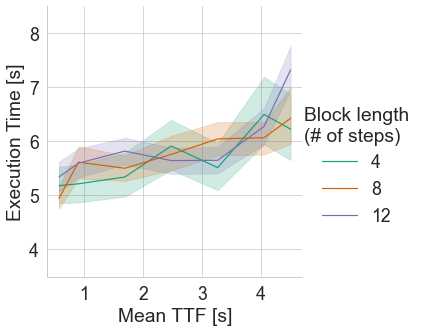
\includegraphics[height=13em]{./Figs/2021Impact/ttf_vs_exectime_per_block}
        \caption{%
            \gls{TTF} vs average execution time, grouped by block length.
            Transparent bands indicate \SI{95}{\percent} \glspl{CI}.
        }\label{fig:ttfvsexectime:block}
    \end{subfigure}%
    \hfill%
    \begin{subfigure}[t]{0.45\textwidth}
        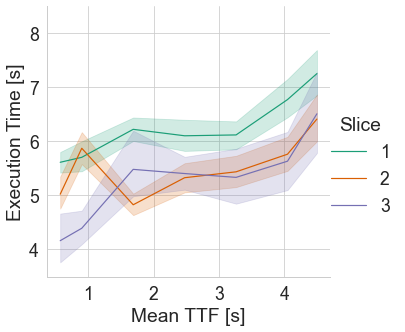
\includegraphics[height=13em]{./Figs/2021Impact/ttf_vs_exectime_per_slice}
        \caption{%
            \gls{TTF} vs average execution time, grouped by step slice in a block.
%            Slice \num{1} corresponds to steps \numrange{1}{4}, \num{2} to steps \numrange{5}{8}, and \num{3} to steps \numrange{9}{12} in a block.
%            Blocks with \num{4} steps only contribute to slice \num{1}, and blocks with \num{8} steps to slices \num{1} and \num{2}.
            Transparent bands indicate \SI{95}{\percent} \glspl{CI}.
        }\label{fig:ttfvsexectime:slice}
    \end{subfigure}%
    \caption{Effects of perceived \gls{TTF} on measured step execution times by participants.}\label{fig:ttfvsexectime}
\end{figure*}

\Cref{fig:ttfvsexectime} shows effects on the measured execution times of participants as perceived \gls{TTF} increased.
These results have been grouped by block length (\cref{fig:ttfvsexectime:block}), showing the cumulative effects of delay over series of steps, and slice number (\cref{fig:ttfvsexectime:slice}), showing the evolution of these effects within a series of steps at the same level of impairment.

\cref{fig:ttfvsexectime:block} shows that as system responsiveness decreased, the speed at which participants completed instructions tended to slow down.
Compared to the unimpaired case, participants were on average \SI{12}{\percent} slower when subject to a mean \gls{TTF} of \SI{2.475}{\second}, and \num{26} percentage points slower at a mean \gls{TTF} of \SI{4.5}{\second}.
\Cref{fig:ttfvsexectime:block} illustrates this effect clearly;
for all block lengths, as \gls{TTF} grows we see an accompanying increase in execution times.
Moreover, this effect seemed stronger for longer blocks at higher levels of impairment, indicating a slow-down which compounds with the number of steps.
Note that by measuring \emph{step execution time} we are \emph{per se} compensating for the added delay in the measure, and thus this trend must result from the participants' behavioral slow-down as a response to the perceived increase in \gls{TTF}.
This was confirmed through an \gls{ANOVA}~\cite{fujikoshi1993two} including factors of block length and \gls{TTF}; significant effects were found for both factors and their interaction (\ensuremath{p < 0.01}).

On the other hand, in \cref{fig:ttfvsexectime:slice} we observe the evolution of execution times over \emph{slices} of \num{4} steps within blocks.
This figure illustrates how, at the lowest levels of impairment, users tended to get faster as the task progressed.
At the lowest \gls{TTF}, the average execution time of steps \num{9} to \num{12} in a block was roughly \textasciitilde\SI{26}{\percent} lower than for steps \num{1} to \num{4}.
However, this effect is strongly dampened at higher levels of impairment, with the difference between the average execution times of steps in slices \num{2} and \num{3} basically disappearing at the highest \gls{TTF}.
This was also confirmed through an \gls{ANOVA} on factors slice and \gls{TTF}, finding significant (\ensuremath{p < 0.01}) for both factors and their interaction.

\begin{figure}
    \begin{minipage}[t]{.45\textwidth}
        \centering
        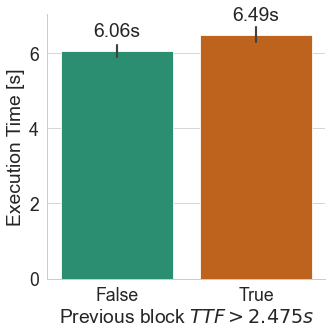
\includegraphics[height=13em]{Figs/2021Impact/previousblock_vs_exectime}
        \caption{Mean execution time of the first slice of steps in a block, grouped by \acs{TTF} of the block immediately preceding the current one.}\label{fig:prevblockvsexectime}
    \end{minipage}%
    \hfill%
    \begin{minipage}[t]{.45\textwidth}
        \centering
        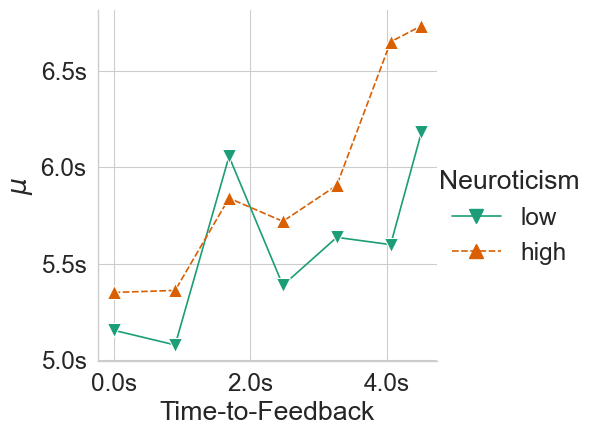
\includegraphics[height=13em]{publications/2023EdgeDroid2/figs/new_model/mu_fits_exgaussian_slice0}
        \caption{%
            Illustration of the effect of neuroticism on the \ensuremath{\mu} parameter of \acs{exGaussian} distributions fitted to the execution times of steps in slice \num{1}.
            Fits were achieved through \gls{MLE}.
            Figure originally published in \cref{paper:olguinmunoz2023realistic}
        }\label{fig:ttfvsexgaussianmu}
    \end{minipage}
\end{figure}

As mentioned before, we found that the effects of system responsiveness on execution times lingered on after the system moved to a different level of impairment.
\Cref{fig:prevblockvsexectime} illustrates this effect.
On average, the mean execution time of the first four steps of blocks was roughly \SI{7}{\percent} lower when the previous block was at a \ensuremath{TTF \leq \SI{2.475}{\second}} compared to when the previous block was at a \ensuremath{TTF > \SI{2.475}{\second}} (single-tailed \ensuremath{p < 0.001}).

Analyses of the correlation between individual subject differences and the above effects highlighted the \gls{BFI} trait of \emph{neuroticism} as an important modulating factor.
This trait has been linked to low tolerance for stress, high emotional reactivity, as well as higher rates of \emph{delay discounting}~\cite{hirsh2008delay}.
Out of the three components identified by a \gls{PCA}, which cumulatively accounted for \textasciitilde\SI{73}{\percent} of the variance in the execution time results, neuroticism was present in the first two.
Individual neuroticism scores were found to significantly linearly correlate (\ensuremath{rho = 0.418}, two-tailed \ensuremath{p < 0.05}) with measured execution times at high \glspl{TTF}.

Finally, we found that execution times were well-fit by \gls{exGaussian} distributions.
Previous research has established strong arguments for the use of this distribution for the modeling of human reaction times and the timings of human actions~\cite{rohrer1994analysis,palmer2011what,marmolejo_ramos2022generalised}.
When grouping execution times by low/high neuroticism\footnote{%
    \emph{Low} refers to values less than the middle value obtainable for neuroticism in the \gls{BFI}; \emph{high} to values greater than or equal to it.
}, \gls{TTF}, and slice, the best fit statistic obtained using a Kolmogorov-Smirnov goodness-of-fit test~\cite{massey_jr1951kolmogorov} was \num{0.028}, with a \ensuremath{p}-value of \num{0.999}.
The effects of neuroticism were most easily observed in the \ensuremath{\mu} parameter and the tails of the fitted distribution;
an example of this can be observed in \cref{fig:ttfvsexgaussianmu}.
There is a clear and direct correlation between higher neuroticism and higher \ensuremath{\mu} values and longer tails.

\subsubsection{Implications for \glsfmtshort{WCA}}

The findings presented above reveal interesting implications for the design and optimization of \gls{WCA} applications.
The noticeable slow-down in user behavior as a response to a decrease in system responsiveness leads to extended application lifetimes even for brief periods of impairment.
This effect is compounded by the persistence of the slow-down effect for a certain period even after the system returns to an improved level of responsiveness.
As a result, this could have unconventional consequences for resource allocation, particularly in multi-tenant deployment and cases where users may be able to finish their task before the effects of slow-down subside.

In such instances, it might be more efficient not to redirect resources to the impaired application, as equitable degradation may not necessarily benefit the system as a whole.
It could even be more beneficial to allocate resources \emph{away} from the impaired application to ensure optimal system responsiveness for other tenants in the system.
This unconventional approach to resource allocation can potentially improve the overall system performance and provide better average \gls{QoE} and \gls{QoS}.

However, the implications mentioned above are purely speculative, and an experimental approach is required to accurately study the consequences of these results.
The complexity of \gls{WCA} application systems makes it challenging to predict the outcomes of resource allocation strategies, and experimentation is necessary to confirm or reject these speculations.

\subsection{A new model of human behavior in \acs{WCA}}

\cref{paper:olguinmunoz2023realistic} discusses the elaboration of a model of human behavior for \gls{WCA}.
Built upon the data and results from \cref{paper:olguinmunoz2021impact}, our model is capable of dynamically generating realistic predictions of execution times for steps in a \gls{WCA} based on historical system state data and a parameterized level of neuroticism.
Furthermore, we implement a new version of the EdgeDroid tool capable of using this new model, together with a novel procedure for the generation of realistic synthetic traces of frames for \gls{WCA}, to provide a fully end-to-end emulation of a human in the context of these systems.

\subsubsection{Design of a realistic model for human timings in \gls{WCA}}

Our current model of human behavior has a limitation that we need to address.
The model we have discussed so far emulates a rigid and unyielding human who is not affected by low responsiveness in the system.
This is not an accurate representation of real human behavior, and in the following we present a more realistic human model that takes into consideration the perceived feedback latency and its effects on human reactions.

Our new model is based on the comprehensive study of human behavior in the presence of feedback latency outlined in \cref{paper:olguinmunoz2021impact}, and has significant implications for the optimization of edge computing systems.
By incorporating a more accurate representation of human behavior into our methodology, we can better assess the impact of system design choices on the end-user experience.
This, in turn, enables future research into optimization strategies that are more effective at improving the overall quality of service for edge computing applications.

\medskip
As discussed in \cref{impact:results}, the execution time for a step depends not only on the most recent perceived \gls{TTF}, but also on how long the system has been in the current level of responsiveness.
Moreover, as shown in \cref{fig:prevblockvsexectime}, the effects of reduced system responsiveness on generated execution times must be taken into consideration even after the system transitions into a more responsive state.
All of these effects are also modulated by neuroticism, adding both another layer of complexity and a means of parameterizing the model.

Our new timing model generates realistic execution times for each step by taking two inputs: the most recent measured \gls{TTF} and a level of normalized neuroticism.
The model is stateful and calculates a weighted average of the 12 most recent \glspl{TTF}, with the most recent step accounting for approximately \SI{50}{\percent} of the weighted result.
The resulting weighted rolling \gls{TTF} is then used to look up potential values for the execution time in the original data and generate a realistic execution time for the step based on the selected level of neuroticism.

To achieve this, the original data from the \num{40} independent repetitions of the LEGO task from \cref{paper:olguinmunoz2021impact} is pre-processed using the same rolling weighted average formula and binned into \num{14} bins corresponding to the seven quantiles for weighted TTF and two levels of neuroticism.
During runtime, the weighted \gls{TTF} calculated is matched to the corresponding bin of samples, which are then filtered based on the selected level of neuroticism.
The execution time is generated either by directly sampling the execution time values from the selected samples or by fitting a theoretical \gls{exGaussian} distribution to these values and then sampling the distribution instead.

\begin{figure}[tb]
    \centering
    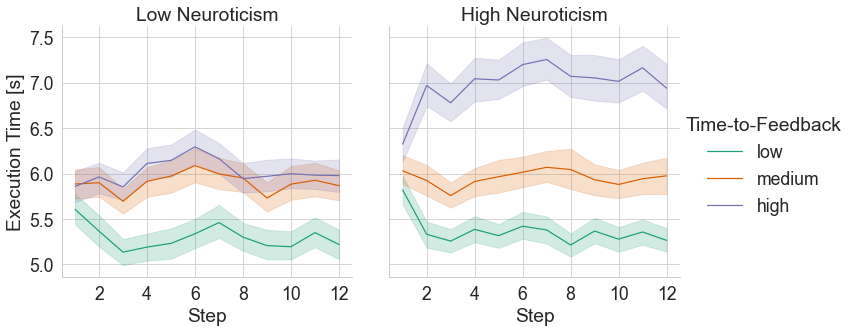
\includegraphics[width=\textwidth]{Figs/2023EdgeDroid2/model_exectime_over_steps}
    \caption{
        Illustration of the execution times output by the model at fixed values of \glspl{TTF}, over a series of steps, parameterized by levels of neuroticism.
        Shaded bands indicate \SI{95}{\percent} \glspl{CI}.
    }\label{fig:model:exectimesoversteps}
\end{figure}

\begin{figure}
    \begin{minipage}[t]{.45\textwidth}
        \centering
        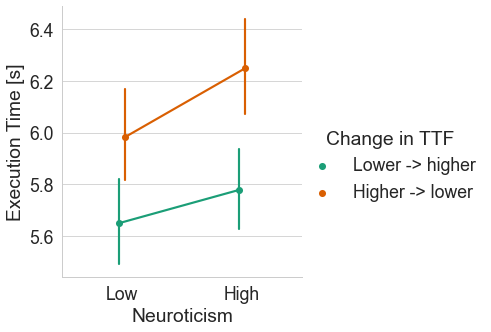
\includegraphics[width=\textwidth]{Figs/2023EdgeDroid2/model_exectimes_transition}
        \caption{%
            Mean execution times generated by the model after a single step at a \gls{TTF} of \SI{2.5}{\second} preceded by a sequence of \num{25} steps at fixed lower (instantaneous feedback) or higher (\SI{5}{\second}) \gls{TTF}.
            Errorbars indicate \SI{95}{\percent} \glspl{CI}.
        }\label{fig:model:exectimestransitions}
    \end{minipage}%
    \hfill%
    \begin{minipage}[t]{.45\textwidth}
        \centering
        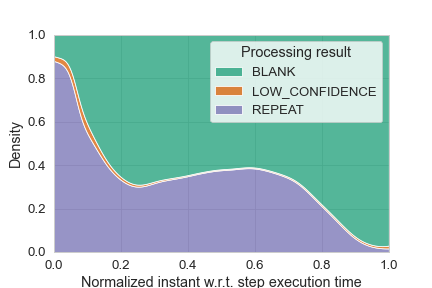
\includegraphics[width=\textwidth]{publications/2023EdgeDroid2/model_data/frame_probabilities}
        \caption{%
            Distribution of processing results for frames captured during the execution of steps in the LEGO task.
            Note that \emph{Success} results are not included since by definition \ensuremath{P(\text{Success}|t_\text{norm}) = 1.0} for all normalized instants \ensuremath{t_\text{norm} \geq 1.0}.
        }\label{fig:modelframes}
    \end{minipage}
\end{figure}


\Cref{fig:model:exectimesoversteps,fig:model:exectimestransitions} illustrate the adherence of the model to the conclusions obtained from our work in \cref{paper:olguinmunoz2021impact}.
\Cref{fig:model:exectimesoversteps} shows the output of the execution time model described above over a series of steps at three levels of \gls{TTF};
\emph{low} (instantaneous feedback), \emph{medium} (\SI{2.5}{\second}), and \emph{high} (\SI{5}{\second}).
When the system is highly responsive (low \glspl{TTF}), the model tends to speed up as the task progresses.
Conversely, at high levels of impairment, execution times depend on strongly on the parameterized level of neuroticism;
as concluded from our previous discussion, higher neuroticism leads to a stronger reaction to reduced responsiveness and subsequently to longer execution times.

In \cref{fig:model:exectimestransitions}, moreover, we present the lingering effects of reduced system responsiveness on \glspl{TTF} generated after the system returns to a more responsive state.
These results were generated by first feeding a sequence of \num{25} identical \glspl{TTF} to the model, with values of either \SI{0}{\second} (i.e.\ instantaneous feedback) or \SI{5}{\second}.
Next, a single \gls{TTF} of \SI{2.5}{\second} was fed to the model, and the generated execution time was recorded.
This procedure was repeated \num{600} times.
As expected from our discussion in \cref{impact:results}, transitions from a higher (\SI{5}{\second}) \gls{TTF} resulted in noticeably inflated execution times (\ensuremath{+\SI{8.5}{\percent}} at a high level of neuroticism) for the first step at \SI{2.5}{\second} \gls{TTF} compared to when the transition was from a lower \gls{TTF}.

\subsubsection{Procedural generation of dynamic traces of video frames for \acs{WCA}}\label{model:traces}

Our design for a procedure for the generation of synthetic yet realistic traces of video inputs for \gls{WCA} follows a stochastic approach.
Analysis of the evolution of the distribution of processing results of frames over their normalized capture instant with respect to step execution time highlighted the pattern illustrated in \cref{fig:modelframes}.
We define the normalized capture instant \ensuremath{t_\text{norm}} for each frame as the timestamp at which it was captured with respect to the beginning of the step, normalized by the total execution time of the same step.
The distribution of the four possible categories of outputs of the \gls{CV} algorithm in the Gabriel LEGO Task~\cite{chen2018application} for each frame (\emph{blank}, i.e.\ no discernible board state, noise; \emph{low confidence}; \emph{success}, a frame which triggers a step transition;
and \emph{repeat}, that is, no change since the last \emph{success} frame) were plotted against normalized capture instants.

These results are then used together with a repository of tagged frames for each step to generate a synthetic trace at runtime by:
\begin{enumerate}
    \item At each sampling instant, calculate the current \ensuremath{t_\text{norm}} with respect to the next desired execution time.
    \item If \ensuremath{t_\text{norm} \geq 1}, send a pre-selected \emph{success}-tagged frame for the current step to the \gls{WCA} backend.
    \item Otherwise, sample the distribution of result categories at the selected \ensuremath{t_\text{norm}} and return a pre-selected frame matching the selected category.
\end{enumerate}

This procedure results in a synthetic stream of frames which generates the same processing load on the backend as a real stream would.
The use of a repository of frames collected from real executions of the task by humans ensures that the load on the network also approximates reality.
More details and a longer discussion on this approach can be found in \cref{paper:olguinmunoz2023realistic}, \cref{ssec:model:frames}.

\subsection{Implications with respect to task completion times}

In this section, we will discuss the implications of the methodology for the optimization of \gls{WCA} applications, in particular when employing the experimental results and the improved model of human timings discussed in \cref{sec:extendingmethodology}.
The discussion presented here is a summarized version of what \cref{paper:olguinmunoz2023realistic} exposes.

The term \emph{task completion time}, in the context of \gls{WCA}, will refer to the time it takes a user to work their way through the task presented by an assistant application.
In \cref{paper:olguinmunoz2023realistic} we refer interchangeably to task completion times as application lifetimes.
This metric directly relates to system resource and energy consumption --- longer task completion times mean that the system is occupied for longer and thus uses more resources.
It thus presents a relatively straightforward yet interesting starting point for the study of the implications of the model on the optimization of \gls{WCA} systems.

\begin{figure}
    \centering
    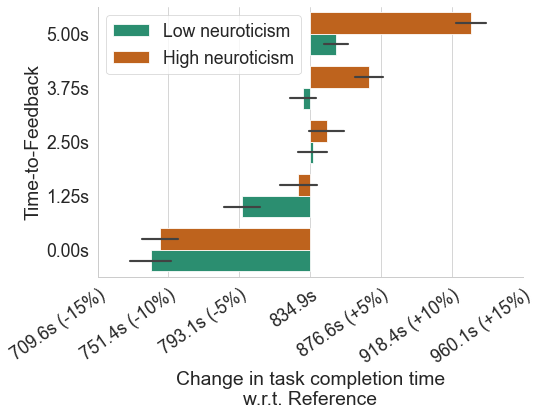
\includegraphics[height=13em]{Figs/2023EdgeDroid2/task_durations_diff}
    \caption{Difference in task completion times of the realistic model with respect to the reference baseline.
    Geometric averages over \num{10} over ten total repetitions per configuration.}\label{fig:taskcompletiontimesdiff}
\end{figure}

The main question we aim to ask relates to the consequences of using our model of human timing behaviors versus using a less realistic approximation.
Specifically, we aim to quantify the difference in task completion times when using the realistic model compared to a baseline which does not take into consideration higher order effects on execution times.
We compare the total task durations of emulated \num{45}-step tasks using the EdgeDroid benchmarking tool with the improved model of human behavior to a baseline model.
Our reference baseline corresponds here to a first order approximation to empirical execution time modeling, using an \gls{exGaussian} distribution fitted to \emph{all} the data points from \cref{paper:olguinmunoz2021impact} (without any grouping) which is randomly sampled to obtain execution time values.
We perform this experiment on the edge computing testbed discussed in \cref{sec:testbed};
for simplicity and to magnify the effects of latency, in this setup we use an \acs{IEEE} \num{802.11}b/g physical layer.

The results of the experiment, as presented in \cref{fig:taskcompletiontimesdiff}, show that there are clear and significant differences in task durations between the models.
At low levels of resource contention, there was a reduction of up to \SI{12}{\percent} in task duration for both levels of neuroticism when using the realistic model.
However, at higher levels of resource contention, the high neuroticism parameterization resulted in task durations that were more than \SI{8}{\percent} longer than the baseline.
These findings demonstrate the importance of using a realistic model of human timing behavior to accurately predict and optimize task completion times.

Overall, this case study highlights the potential benefits of using our methodology coupled with a realistic model of human timing behavior in edge computing systems.
By considering higher order effects on execution times, such as the impact of neuroticism, we can improve the accuracy of our predictions and optimize system performance.
However, it is important to note that the effects of using a realistic model may vary depending on the specific context and task being performed.
Further research is needed to explore the generalizability of our findings and to investigate other factors that may impact task completion times in edge computing systems.

\subsection{Implications with respect to number of samples per step}

In the present section and the following we briefly discuss the implications of our methodology on the optimization potential of number of samples and energy consumption per step, respectively.
Both these analyses depend on an understanding of the tradeoffs between resource consumption and responsiveness in \gls{WCA};
fewer samples per step translates into longer sampling periods, and lower energy consumption tends to be made possible by processing fewer bits of data per step.

We employ in these sections an optimization framework based primarily upon the work of Moothedath et al.~\cite{moothedath2021energy,moothedath2022energy1,moothedath2022energy2}.
The goal of this framework is to balance between increased responsiveness due to higher sampling rates and reduced resource consumption and network congestion caused by excessive sampling.
In general, any objective metric in these applications which relates to sampling and the responsiveness of the system will present itself
as a linear combination between \ensuremath{\mathbb{E}[\mathcal{S}]} and \ensuremath{\mathbb{E}[\mathcal{W}]} plus terms independent of the number of samples or wait time:
\begin{alignat}{1}\label{eq:tradeoff}
    \Rightarrow\mathcal{E}&=\alpha\mathbb{E}[\mathcal{S}]+\beta\mathbb{E}[\mathcal{W}]+C\;
\end{alignat}
The constants \ensuremath{\alpha}, \ensuremath{\beta}, and \ensuremath{C} modify the objective function from one metric to another.

\medskip
For the problem of minimizing the number of samples, an unconstrained optimization of the above equation leads to a single sample at \ensuremath{t \rightarrow \infty} and an infinite wait time.
Thus, a constrained optimization is performed with an upper bound \ensuremath{w_0} for the expected wait time, i.e.\ \ensuremath{\mathbb{E}[\mathcal{W}] \leq w_0}.
The below equation is derived in \cref{paper:olguinmunoz2023realistic} for finding appropriate \ensuremath{\alpha} and \ensuremath{\beta} for this problem:
\begin{alignat}{1}\label{eq:sampling}
\frac{\alpha}{\beta}=\frac{2\sqrt{2}\,w_0^2}{(\mathlarger{\Gamma}(\tfrac{3}{4}))^2\,\sigma}\approx1.9\frac{w_0^2}{\sigma}
\end{alignat}
This solution assumes execution times distributed according to a Rayleigh distribution with parameter \ensuremath{\sigma}.
\ensuremath{\mathlarger{\Gamma}(x)} is the Gamma function.
Note that the full derivation and explanation of this solution is out of the scope of this summary;
please refer to the paper and its appendix for a detailed discussion on this optimization approach.

A reference scheme from~\cite{wang2019towards} is introduced which adjusts the sampling rate at each sampling instant \ensuremath{t} according to the estimated likelihood of the user finishing the step.
The scheme uses a static Gaussian distribution for all steps.

We compare the effects of the optimization approach with the timing models to the reference scheme.
We implement a sample-count-optimized aperiodic sampling scheme using \cref{eq:sampling} to determine the optimum sampling instants and the values for \ensuremath{\alpha} and \ensuremath{\beta}.
The scheme includes an embedded human timing model that measures the perceived system responsiveness and updates the \ensuremath{\sigma} parameter at every step.
The reference scheme is implemented using the Gaussian distribution fitted to the execution times in \cref{paper:olguinmunoz2021impact}.

\begin{figure}
    \centering
    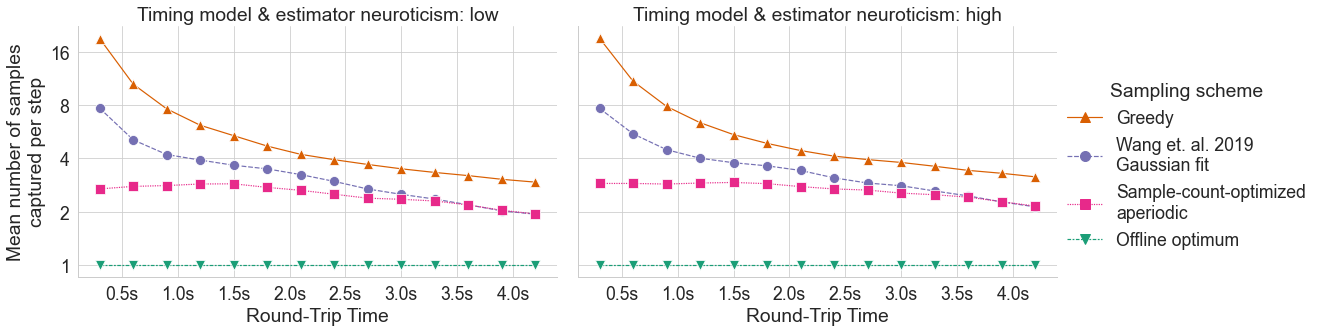
\includegraphics[width=\textwidth]{publications/2023EdgeDroid2/figs/new_model/sampling_optimization}
    \caption{%
        Round-trip time versus mean number of captured samples per step (logarithmic Y-axis).
        Error bars indicate \SI{95}{\percent} \glspl{CI}.
        Figure originally published in \cref{paper:olguinmunoz2023realistic}.
    }\label{fig:samplingresults}
\end{figure}

Simulations were performed in Python to test different sampling schemes.
The results from these simulations are presented in \Cref{fig:samplingresults}.
The figure compares the performance of four sampling schemes:
\begin{inlineenum}
    \item the sample-count-optimized approach described above
    \item \citeauthor{wang2019towards}s adaptive approach based on a Gaussian distribution
    \item a \emph{greedy}, completely unoptimized approach
    \item an \emph{offline optimum} scheme which perfectly predicts execution times in order to only sample once per step
\end{inlineenum}.

The results indicate that the sample-count-optimized aperiodic scheme results in a lower mean number of samples per step compared to the reference scheme proposed by \citeauthor{wang2019towards}.
This was achieved while still satisfying the expected wait time bound.

The performance of the sample-count-optimized aperiodic scheme was further enhanced by incorporating the timing model that reflects human behavior.
The timing model allows for a more precise optimization of the sampling rate in \gls{WCA} applications, which minimizes the number of samples needed while still meeting the responsiveness requirements.
These results highlight the effectiveness of the optimization approach and the significance of the timing model in optimizing sampling rates, as well as provide further validation of our methodology.


\subsection{Implications with respect to raw energy consumption}\label{ssec:implications:energy}

We also optimize for energy consumption in \gls{WCA}.
Energy consumption in these applications depends on various factors such as the number of samples captured, communication power and delays, among others.
Hence, minimizing the number of samples captured is not a guarantee of reducing energy consumption.
We therefore take the general solution for \cref{eq:tradeoff} and find the appropriate values of \ensuremath{\alpha} and \ensuremath{\beta} to minimize the energy consumed per step, represented by \ensuremath{\mathcal{E}=E}.
With feedback given even to the discarded samples in our model and communication delay defined as the total delay in either direction, we have,
\begin{alignat}{2}
    \mathrm{E}=&\;\mathcal{S}\tau_cP_c+(\mathcal{T}+\mathcal{W}+\tau_\mathrm{p}+\tau_\mathrm{c}-\mathcal{S}\tau_c)P_0\nonumber\\
    % &=s\tau_c(P_c-P_0^{(t)})+wP_0^{(t)}+(\tau+\tau_c+\tau_p) P_0^{(t)}+\tau_cP_c\\
    =&\;\tau_{\text{c}}(P_{\text{c}} -P_0)\mathcal{S}+\mathcal{W}P_0+(\mathcal{T}+\tau_{\text{p}} +\tau_{\text{c}}) P_0\nonumber\\
    &\Rightarrow \alpha=\tau_{\text{c}}(P_{\text{c}} -P_0),\text{ and }\beta=P_0
\end{alignat}
\( \tau_\text{p} \) and \( \tau_\text{c} \) correspond to the processing and two-way communication delay for each sample.
\( P_\text{c} \) and \( P_0 \) correspond to the communication and idle power, respectively, of the \gls{WCA} client device.

We perform an experiment to implement the energy-optimized aperiodic sampling scheme, replacing the sample-count-optimized sampling scheme.
The energy-optimized scheme uses the calculated values of \ensuremath{\alpha} and \ensuremath{\beta} to minimize energy consumption.
The values of communication power, \ensuremath{P_{\text{c}}}, and idle power, \ensuremath{P_0}, are estimated from previous research.
The processing delay, \ensuremath{\tau_{\text{p}}}, is set to a constant value across all experiments, and the communication delay, \ensuremath{\tau_{\text{c}}}, is calculated as the \gls{RTT} minus the processing delay.
As before, the optimized sampling scheme includes an embedded timing model to provide updated predictions for \ensuremath{\sigma} at every step.

\begin{figure}
    \centering
    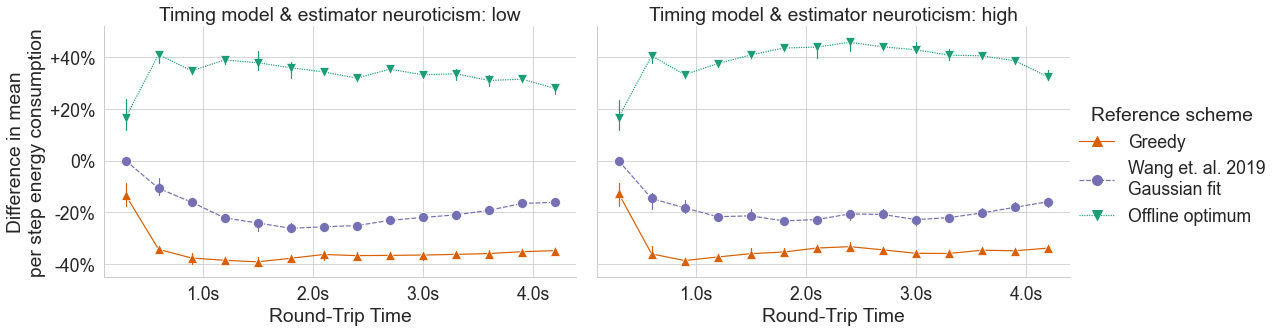
\includegraphics[width=\textwidth]{publications/2023EdgeDroid2/figs/new_model/energy_optimization_diff}
    \caption{%
        Percentage difference in mean per step energy consumption by the energy-optimized sampling scheme with respect to the three reference schemes.
        Error bars indicate \SI{95}{\percent} \glspl{CI}, calculated using a two-sided t-test.
        Figure originally published in \cref{paper:olguinmunoz2023realistic}.
    }\label{fig:energyresults}
\end{figure}

The results of our experiments, illustrated partially in \cref{fig:energyresults}, show that this energy-optimized scheme outperforms the reference schemes, with a significant reductions in energy consumption.
Our approach is consistently consumes \SI{20}{\percent} less energy than \textcite{wang2019towards}'s approach, and is able to achieve up energy savings of up to \SI{40}{\percent} with respect to the greedy scheme.
Furthermore, our approach is more consistent and reliable, exhibiting a flat curve of energy consumption much akin to that of the offline optimum in behavior.

Our findings have important implications for the development and deployment of \gls{WCA} systems.
We have demonstrated that it is possible to significantly reduce the energy consumption of these systems while still maintaining a reasonable \gls{RTT}.
This can help extend the battery life of wearable devices, making  systems more practical and usable for a wider range of users.
The results of this study can serve as a valuable reference for future work in energy optimization for \acl{WCA} systems.
